%\documentclass[sigplan]{acmart}
\documentclass[sigplan,screen]{acmart}
\usepackage[utf8]{inputenc}
\usepackage{alltt,xcolor}
%\usepackage{flafter}
\usepackage{listings}
\usepackage{comment}
\usepackage{todonotes}
\usepackage{url}

%%
%% \BibTeX command to typeset BibTeX logo in the docs
\AtBeginDocument{%
  \providecommand\BibTeX{{%
    \normalfont B\kern-0.5em{\scshape i\kern-0.25em b}\kern-0.8em\TeX}}}

%% If you see 'ACMUNKNOWN' in the 'setcopyright' statement below,
%%% please first submit your publishing-rights agreement with ACM (follow link on submission page).
%%% Then please update our instructions page and copy-and-paste the NEW commands into your article.
%%% Please contact us in case of questions; allow up to 10 min for the system to propagate the information.
%%%
%%% The following is specific to SLE '19 and the paper
%%% 'From DSL Specification to Interactive Computer Programming Environment'
%%% by Pierre Jeanjean, Benoit Combemale, and Olivier Barais.
%%%
\setcopyright{acmlicensed}
\acmPrice{15.00}
\acmDOI{10.1145/3357766.3359540}
\acmYear{2019}
\copyrightyear{2019}
\acmISBN{978-1-4503-6981-7/19/10}
\acmConference[SLE '19]{Proceedings of the 12th ACM SIGPLAN International Conference on Software Language Engineering}{October 20--22, 2019}{Athens, Greece}
\acmBooktitle{Proceedings of the 12th ACM SIGPLAN International Conference on Software Language Engineering (SLE '19), October 20--22, 2019, Athens, Greece}

\colorlet{punct}{red!60!black}
\definecolor{background}{HTML}{EEEEEE}
\definecolor{delim}{RGB}{20,105,176}
\colorlet{numb}{magenta!60!black}

\begin{document}

\title{From DSL Specification to Interactive Computer Programming Environment}
% Automatic synthesis of REPL from Language interpreter
% Systematic REPL generation for visitor-based DSL
% 


\author{Pierre Jeanjean}
\affiliation{%
  \institution{Inria, Univ Rennes, CNRS, IRISA}
  \city{Rennes}
  \country{France}}
\email{pierre.jeanjean@inria.fr}

\author{Benoit Combemale}
\affiliation{%
  \institution{University of Toulouse}
  \city{Toulouse}
  \country{France}}
\email{benoit.combemale@irit.fr}

\author{Olivier Barais}
\affiliation{%
  \institution{Univ Rennes, Inria, CNRS, IRISA}
  \city{Rennes}
  \country{France}}
\email{olivier.barais@irisa.fr}

%%
%% By default, the full list of authors will be used in the page
%% headers. Often, this list is too long, and will overlap
%% other information printed in the page headers. This command allows
%% the author to define a more concise list
%% of authors' names for this purpose.
\renewcommand{\shortauthors}{Pierre Jeanjean, Benoit Combemale and Olivier Barais}

\begin{abstract}
% Context
The adoption of Domain-Specific Languages (DSLs) relies on the capacity of language workbenches to automate the development of advanced and customized environments. 
%
%Problem
While DSLs are usually well tailored for the main scenarios, the cost of developing mature tools prevents the ability to develop additional capabilities for alternative scenarios targeting specific tasks (e.g., API testing) or stakeholders (e.g., education). 
%
%Approach
In this paper, we propose an approach to automatically generate interactive computer programming environments from existing specifications of textual interpreted DSLs. 
%
%More specifically, we consider an EMF-based language complemented with an operational semantics in the form of a visitor (or using the native EMF Switch), and automatically generate a REPL engine. 
%
%Scope of applicability: textual grammar-based language, explicit control flow, operational semantics in the form of a well-defined (top-down) interpreter or visitor, 
%
%The approach reifies the relevant abstractions to use when specifying the DSL, and use a combination of static analysis and language transformations to automate the translation of both the language syntax and semantics. The syntax is converted such as it is possible to load partial program limited to single statements, and the language interpreter is turn into an Read-Eval-Print Loop (REPL) engine. Hence, we provide the required generative approach to automate the integration into a ready-to-use interactive computer programming environments. 
%
%Results
The approach provides abstractions to complement the DSL specification, and combines static analysis and language transformations to automate the transformation of the language syntax, the execution state and the execution semantics.
%
%Conclusion
We evaluate the approach over a representative set of DSLs, and demonstrate the ability to automatically transform a textual syntax to load partial programs limited to a single statement, and to derive a Read-Eval-Print-Loop (REPL) from the specification of a language interpreter.
%
%While applicable to a broad range of textual and interpreted languages, our approach not only provide an REPL engine for free, but also transform the syntax such as it is possible to load partial model limited to single statements.

\end{abstract}

%%
%% The code below is generated by the tool at http://dl.acm.org/ccs.cfm.
%% Please copy and paste the code instead of the example below.
%%
\begin{CCSXML}
<ccs2012>
<concept>
<concept_id>10011007.10011006.10011050.10011017</concept_id>
<concept_desc>Software and its engineering~Domain specific languages</concept_desc>
<concept_significance>500</concept_significance>
</concept>
</ccs2012>
\end{CCSXML}

\ccsdesc[500]{Software and its engineering~Domain specific languages}

\lstdefinelanguage{json}{
    basicstyle=\normalfont\ttfamily,
    numbers=left,
    numberstyle=\scriptsize,
    stepnumber=1,
    numbersep=8pt,
    showstringspaces=false,
    breaklines=true,
    frame=lines,
    backgroundcolor=\color{background},
    literate=
     *{0}{{{\color{numb}0}}}{1}
      {1}{{{\color{numb}1}}}{1}
      {2}{{{\color{numb}2}}}{1}
      {3}{{{\color{numb}3}}}{1}
      {4}{{{\color{numb}4}}}{1}
      {5}{{{\color{numb}5}}}{1}
      {6}{{{\color{numb}6}}}{1}
      {7}{{{\color{numb}7}}}{1}
      {8}{{{\color{numb}8}}}{1}
      {9}{{{\color{numb}9}}}{1}
      {:}{{{\color{punct}{:}}}}{1}
      {,}{{{\color{punct}{,}}}}{1}
      {\{}{{{\color{delim}{\{}}}}{1}
      {\}}{{{\color{delim}{\}}}}}{1}
      {[}{{{\color{delim}{[}}}}{1}
      {]}{{{\color{delim}{]}}}}{1},
}


%%
%% Keywords. The author(s) should pick words that accurately describe
%% the work being presented. Separate the keywords with commas.
\keywords{repl, language engineering, domain specific languages}

%% A "teaser" image appears between the author and affiliation
%% information and the body of the document, and typically spans the
%% page.
%\begin{teaserfigure}
%  \includegraphics[width=\textwidth]{sampleteaser}
%  \caption{Seattle Mariners at Spring Training, 2010.}
%  \Description{Enjoying the baseball game from the third-base
%  seats. Ichiro Suzuki preparing to bat.}
%  \label{fig:teaser}
%\end{teaserfigure}

\maketitle

\section{Introduction}

% Context
Domain-Specific Languages (DSLs) are software languages specifically tailored (e.g., syntax, semantics and tools) for a given problem space. While attractive in many application domains, the success of DSLs relies on the ability of language workbenches to support their specifications and automate the development of advanced and customized tools. In the last decade, various language workbenches have been proposed, with different facilities, formalisms and underlying implementation frameworks \cite{DBLP:journals/cl/ErdwegSVTBCGH0L15}.	

% Problem
While covering together a broad range of programming and modeling facilities, language workbenches face interoperability issues \cite{coulon:hal-01889155}. In particular language workbenches are usually well equipped in terms of formalisms, implementation frameworks and generative approaches to eventually obtain a fine-tuned specific set of tools, initially chosen for targeting the main scenarios. But then, it often fails to encompass other forms of implementation that would fit alternative scenarios. DSL specifications are hardly reusable for driving the development of various forms of DSL environments \cite{acher:hal-01061576}.

For example, while nowadays comprehensive BNF-based interpreted language specifications would drive the development of comprehensive DSL environments, it is hard to drive the development of alternate environments such as interactive computer programming environments. They are interactive environments that help to document (\emph{e.g.,} Jupyter\footnote{cf. \url{https://jupyter.org/}} \cite{Shen14}), to evaluate APIs (\cite{DBLP:conf/models/TombelleV06,sarid2016api}), to teach \cite{Allen:2002:DLP:563340.563395,Gray:2003:PGI:949344.949394,10.1007/BFb0033856}, to share knowledge (\emph{e.g.,} in science \cite{4160251,Perkel19}), or for arts \cite{quteprints31056}. In practice, most of today's DSL specifications have a single execution entry-point responsible for executing the whole program. Interactive environments support multiple entry points, with different strategies for managing the execution context and flow. Beyond the parser itself, the execution engine must turn into a \textit{Read-Eval-Print Loop} (REPL), that repeatedly reads an input from the user, evaluates it and prints a result. One of the main advantages of using a development environment that includes a REPL is to be able to write and execute a program piece by piece.

% Appraoch
In this paper, we propose an approach to automatically generate interactive computer programming environments from existing specifications of textual interpreted DSLs. More specifically, the approach reifies the relevant abstractions to use when specifying the DSL, and use a combination of static analysis and language transformations to automate the translation of both the language syntax and semantics. The syntax is converted such as it is possible to load partial program limited to single statements, and the semantics in the form of a language interpreter is turned into a REPL. Hence, we provide the required generative approach to automate the integration into a ready-to-use interactive computer programming environments in the form of both a language shell into Eclipse, and a specific Notebook (\emph{a la} Jupyter). 

We provide an implementation of the approach as a prototype on top of the Eclipse Modeling Framework \cite{steinberg2008emf}, which includes Ecore\footnote{cf. \url{https://www.eclipse.org/modeling/emf/}} for the syntax definition, Xtext\footnote{cf. \url{https://www.eclipse.org/Xtext}} for the textual syntax definition, and ALE\footnote{cf. \url{http://gemoc.org/ale-lang}} for the operational semantics definition. The approach would be similarly applied to other alternatives within EMF (\emph{e.g.,} Java or ATL interpreters, or using the native EMF Switch), or other implementation frameworks (\emph{e.g.}, Truffle-based interpreter). The approach applies to any DSL specification with a BNF definition of the syntax which includes an explicit definition of the execution flow, and an operational semantics specification in the form of a well-defined (top-down) interpreter or visitor.  

% Evaluation
We apply our approach on several DSLs, namely \emph{Logo}, \emph{MiniJava} and \emph{ThingML}~\cite{Harrand:2016:TLC:2976767.2976812}%, and demonstrate its applicability on a broad range of languages
. According to the different paradigms (\emph{e.g.}, control-flow vs. data-flow), we discuss the different ways to operate our approach and provide relevant interactive computer programming environments. 

% Conclusion
Hence, we provide a well-defined and automatic approach for complementing a modeling environment with an interactive computer programming environment. The resulting environment also provides several extension points to possibly customize the execution flow. Finally, we discuss several perspectives, including the deployment on web technologies.	


% Sectionning

The remainder of this paper is structured as follows. We motivate our contribution in Section \ref{motiv}, and introduce an illustrative example used throughout the paper. Section \ref{approach} presents an overview of our approach, while Section \ref{transformation} gives the details of the transformation of the syntax and the semantics. We present an evaluation of our approach in Section \ref{sec:evaluation}, and discuss related works in Section \ref{sec:rw}. Finally, a conclusion and future research directions are presented in Section \ref{sec:conclusion}.


\section{Background and Motivation}
\label{motiv}

The main objective of our approach is to automatically generate an interactive computer programming environment from a DSL specification initially designed to drive the development of a comprehensive DSL environment with an advanced editor, a regular interpreter, etc. Such a specification usually involves a syntax definition, e.g., in the form of a BNF-like description, and a definition of the semantics, e.g., an operational semantics in the form of an interpreter (or any variant such as a visitor pattern). A language definition also includes static semantics, which define all the context conditions that ensure statically correct conforming programs. In such a definition, the language usually encompasses a single execution entry point, a finely tuned execution context and an interpreter which defines a particular traversal of a given syntax tree to manipulate and update the execution context over the execution. 

Such a language definition is now well supported by advanced language workbenches that help language engineers to develop language tools such as structured editors, debuggers and simulators. For instance, tools like Xtext\footnote{cf. \url{https://www.eclipse.org/Xtext/}} support the generation of an advanced editor with a parser, syntactic validation, and all the features of modern code editors (\emph{e.g.,} syntax coloring, auto completion, etc.). The GEMOC Studio\footnote{cf. \url{http://gemoc.org/studio.html}} helps to complement the language tooling with advanced execution engines and debugging facilities. Other language workbenches (\emph{e.g.,} MPS, Rascal, Spoofax) offer similar facilities \cite{DBLP:journals/cl/ErdwegSVTBCGH0L15}. Most of these workbenches are now mature enough for being included in industrial settings, and allow language engineers to automate the development of the tools for the main scenarios of the expected language users. 

Let us consider for example the language \textit{Logo}\footnote{cf. \url{https://en.wikipedia.org/wiki/Logo_(program}}. \textit{Logo} is an educational language whose main focus is the animation of turtle graphics. As such, most of the statements are accompanied by a feedback which is an action from the turtle, and this is part of what makes it interesting for teaching purposes. From a comprehensive definition of the language, it is possible to automatically generate a dedicated and structured editor that supports the definition of complete logo programs, including a functional architecture and an explicit execution flow across the architecture. 

However, it has been recently recognized that the different tasks performed with a given language, possibly by different stakeholders, would require specific language support (\emph{e.g.,} dedicated environments with the right facilities) \cite{acher:hal-01061576}. For instance, while it can be convenient to have a comprehensive editor for editing complex logo programs, one would like access to other kinds of environment such as interactive environments that allow to immediately get the result of the program at the time it is being edited. Such an environment would be very useful for education purposes, such as learning about the language or evaluating existing libraries. Generally speaking, it becomes way easier to introduce a programming language to beginners if they don't have to conform to the structure of an entire program when they want to write their very first instructions~\cite{10.1007/BFb0033856}. \emph{Java} is a perfect example of this~\cite{Gray:2003:PGI:949344.949394,Allen:2002:DLP:563340.563395}, as this is a language that requires to follow a rather complex process to simply print `Hello World!' in a terminal emulator: the programmer needs to define a public class, declare a method both public and static and give it a specific name, while also specifying that it will require a certain type of arguments, before finally writing the very first statement of a program. Of course, the syntax makes perfectly sense, and understanding it will be important in order to learn how to use the language, but it can be detrimental to introduce it during the first glimpse at Java programming. An interactive computer programming environment can be beneficial to simply learn how specific language statements work in practice. In the case of \textit{Logo}, interactive computer programming environments would provide immediate feedback from any statement of the language, and help learning complex concepts. Note that interactive computer programming environments can be also beneficial for experienced language users, in order to test the behavior of code snippets at any time. It makes possible to run processes in an arbitrary order while having access to all the intermediary results, which can be very useful when experiencing a new API. Beyond learning the different facilities provided by the API, it may also help to learn specific protocols in the use of the API. 

Interactive computer programming environment can take various forms, including a basic language shell where single statements can be executed sequentially, based on a global context, and possibly with the history of the intermediate states of the built program. Alternatively, a notebook interface provides a virtual notebook environment used for literate programming. It support the definition of a sequence of pieces of code, with intermediate results, and possibly word processing to document the program. 

In all cases, an interactive computer programming environment requires a language interpreter in the form of a read–eval–print loop (REPL), which is able to execute a program piece by piece.  This requires to support different execution entry-points, and a specific management of the execution context and flow. The context is usually global (though some scoping rules can still apply), and the execution flow is sequential, starting from the starting point defined by the programmer. Other strategies may exist, in particular regarding the execution flow where a specific order may be imposed to keep reproducible executions. 

REPL execution engines offer facilities such as: history of inputs and outputs, input editing and context specific completion over symbols, path names, class names and other objects, as well as help and documentation for commands.

Nowadays, most general purpose languages take these considerations into account, and ship their own REPL implementation: \emph{Python} and \emph{C\#} run in interactive mode by default, \emph{Node.js} can execute the ``repl'' module out of the box, \emph{PHP} can be run as an interactive shell with the switch ``-a'', \emph{Swift} offers a REPL within Xcode, \emph{Ruby} is shipped with the executable ``IRb'', and even \emph{Java} includes its own REPL ``JShell'' since the version~9 of JDK.

While interactive computer programming environments have been specifically developed for general purpose languages, there is currently no approach that helps to turn an existing DSL specification in a way that a complementary interactive environment can be automatically generated. Instead, a new specification must be established for the specific purpose of driving the development of an interactive environment. Hence, the research question (RQ) we address in this paper is the following: 
	\begin{quote}
	RQ: Is it possible to automate the transformation of an existing textual and interpreted DSL specification in such a way that an interactive computer programming environment can be automatically derived? 
	\end{quote}
	
	We consider a DSL specification that includes:
	\begin{itemize}
		\item a syntax described as a grammar defined using a rule language based on "Extended Backus-Naur Form Expressions",
		\item static semantics built from a set of first order logic rules, and
		\item operational semantics based on a \textit{pure} interpreter pattern. \textit{Pure} means that each \textit{interpret} method of the interpreter accesses only the node object 	attributes and the context object attributes.
	\end{itemize}

Our approach provides the required abstractions for complementing an existing DSL specification with the minimal information needed for generating a REPL (\emph{i.e.}, the expected execution entry points and their associated documentation and output messages), and automates the transformation of the DSL specification so that an interactive computer programming environment can be derived. In particular, we automate the transformation of the syntax to parse separate pieces of code, and the semantics to support the execution of single statements according to a specific execution context and flow. We also propose a unified REPL interface in order to derive different kinds of environment, e.g., a language shell and a  notebook interface. 


%%%......................

\begin{comment}

We want to provide language designers with a way to easily obtain a REPL for their languages.
We do not, however, target languages that were made especially with interactivity in mind.
Our intent is not to replace the work that a designer would put into his own interactive language, but to enable the ones working on more traditional DSLs to still obtain some interactivity with minimal effort.
We see several advantages to having a REPL for languages that were not originally intended for this kind of execution:




A REPL can circumvent this by, for example, making the print statement a valid entry-point.
By having access to an interactive environment, it becomes easier to focus on particular matters and to teach in a more incremental way.

In order to better illustrate the educational benefits of having an interactive environment available, we will use the language \textit{Logo}.


 With interactivity, the feedback becomes instantaneous, and the learning can be more incremental by reusing the existing canvas when introducing new concepts.

However, even an experienced language user can find an interest in using a REPL, since it gives the ability to test the behaviour of code snippets or whole methods at any time.
It basically becomes possible to run processes in an arbitrary order while having access to all the intermediary results, which can be very useful when experimenting with an API for example:
In some instance, an API might require to follow a rather complex protocol.
Implementing the right sequence of actions in a working process can be a terrible ordeal if the programmer needs to edit and restart the whole program after each failure.
As such, an interactive interpreter becomes the perfect tool to deal with these situations.

Nowadays, most general purpose programming languages take these considerations into account, and ship their own REPL implementation:
\begin{itemize}
    \item \textit{Python} and \textit{C\#} run in interactive mode by default
    \item \textit{Node.js} can execute the ``repl'' module out of the box
    \item \textit{PHP} can be run as an interactive shell with the switch ``-a''
    \item \textit{Swift} offers a REPL though Xcode
    \item \textit{Ruby} is shipped with the executable ``IRb''
    \item Even \textit{Java} includes its own REPL ``JShell'' since version~9
\end{itemize}

By offering an interactive interpreter, these languages could also be easily integrated in computational notebooks such as \textit{Jupyter}.
As such, they can appeal to new users who have a need for the data analysis tool set provided by these environments.
We would also like to see this kind of deployments for DSLs, and this work is a first step towards this goal.

%\subsection{Problem Statement}

There is no single definition around the notion of REPL, it can range from a rather precise description of the functionalities required as for the scheme programming language to a specific vision as in \url{repl.it}. In this paper, we define the notion of Repl as follows: 

\begin{definition}

\item A REPL is a language interpreter able to execute a program piece by piece, from several different execution entry-points. Its core functionalities are the following: 

%For a language that accepts only models of a specific type as an entry-point, this means that a REPL should be able to execute independent parts of these models (that are of different types) while achieving the same results.

%This is quite straightforward with imperative languages, whose execution is generally based on a visitor pattern:
%\begin{itemize}
%    \item Nodes are executed by their parents, using the provided scope and the results of their leaves
%    \item Executed nodes spread the consequences of their side effects to the scope they received
%\end{itemize}
%By creating and managing a top level scope, a REPL has thus all it needs to execute sub-nodes of a complete model.

%There is however less interest for functional languages, and overall for languages that don't allow for side effects.
%Indeed, since executing instructions have no effect on the execution of future ones, having a single REPL or several interpreters for each part makes no difference.
%Also, if having several entry-points for a language is not even wanted (which is the case for most functional languages, whose every elements are expressions and thus potential entry-points), it is fair to assume that a REPL as we defined it would be useless.

%The usefulness of a REPL for dataflow languages is harder to define.
%Being declarative, dataflow languages don't actually drive the execution and are more of description languages: the user doesn't expect the elements to have an effect on their own, only the whole model is meaningful (this is also a valid point for fully declarative functional languages).
%But the individual semantic of the different elements is indeed used to drive the execution.
%As such, a REPL for an actual dataflow language would try to connect descriptions of parts of a model with a semantic that doesn't make any sense if it is not executed by the whole model.
%It is however easy to imagine two situations in which a REPL would be useful for a dataflow language:
%\begin{itemize}
%    \item In order to describe the dataflow, with a semantic whose only purpose is to create the structure
%    \item In order to drive the execution, with a syntax that aims to actually have an effect on the execution
%\end{itemize}
%Taking all of this into account, we decided to focus our approach on imperative languages using the visitor pattern.




\end{definition} 



\begin{enumerate}
\item History of inputs and outputs.
\item Variables are set for the input expressions and results. These variables are also available in the REPL. 
%\item Levels of REPLs. In many Lisp systems if an error occurs during the reading, evaluation or printing of an expression, the system is not thrown back to the top-level with an error message. Instead a new REPL, one level deeper, is started in the error context. The user can then inspect the problem, fix it and continue - if possible. If an error occurs in such a debug REPL, another REPL, again a level deeper, is started. Often the REPL offers special debug commands.

%\item Error handling. The REPL provides restarts. These restarts can be used, when an error occurs, to go back to a certain REPL level.
\item Input editing and context specific completion over symbols, path names, class names and other objects.
\item Help and documentation for commands.
\end{enumerate}


The important challenge addressed in this paper can thus be reformulated as the following Research Question \textbf{RQ1}. 
Is it possible to automatically extend a language specification including:
\begin{enumerate}
\item the syntax described as a grammar defined using a rule language based on "Extended Backus-Naur Form Expressions".
\item Static semantics built from a set of first order logic rules 
\item the operational semantics based on an \textit{pure} interpreter pattern. \textit{Pure} means that each \textit{interpret} method of the interpreter accesses only to the node object attribute and the context object attribute.  
\end{enumerate}

in order to automatically derive an interactive programming environment for this language?

In particular, this work shows how to automatically transform the grammar specification and the operational semantics definition to support interactive programming environment, and the REPL feature defined above. Based on this work, try to answer the second following research question \textbf{RQ2}: What are the remaining scientific breakthrough for easing the creation of advanced interactive programming environment?

\end{comment}


\section{Approach Overview}
\label{approach}

The main objective of our approach is to automatically transform an existing DSL specification (cf. upper left part in Fig.~\ref{fig:overview}) initially used to drive the development of a comprehensive integrated development environment (cf. lower left part in Fig.~\ref{fig:overview}), into a new one (cf. upper right part in Fig.~\ref{fig:overview}) that can be used to automate the development of interactive computer programming environments (cf. lower right part in Fig.~\ref{fig:overview}). 
%
% the following: from an input that contains the syntax and the operational semantics of a language defined using the Interpreter pattern enriched with a set of metadata used to configure the transformation function, our approach generates a language specialized for REPL execution (Figure~\ref{fig:overview}).
%
\begin{figure*}[htb]
	\centering
	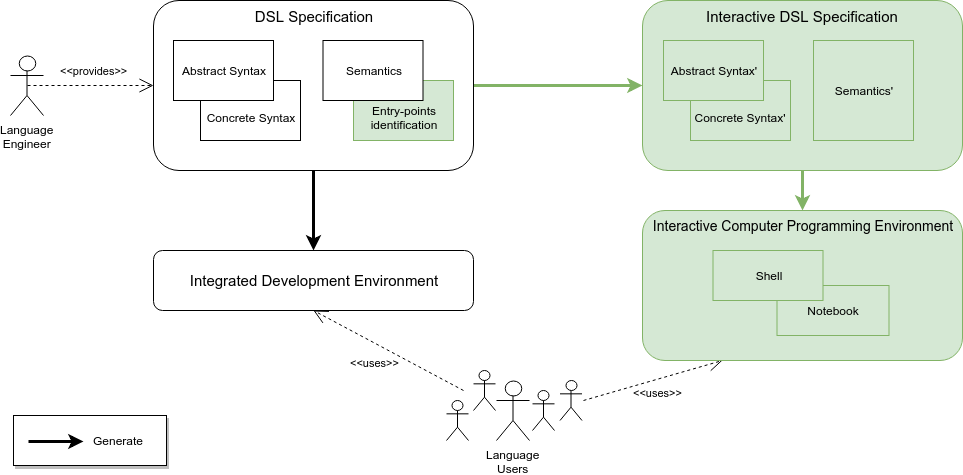
\includegraphics[width=0.7\linewidth]{figures/sle_overview.png}
	\caption{Programming environment generation from DSL specifications}
	\label{fig:overview}
\end{figure*}
%

Since we are aiming for a systematic transformation process, we put some restrictions on the supported DSLs: they need an extended BNF grammar and operational semantics that follow a pure interpreter pattern.
We believe that these characteristics are ones of the most common, and thus that these are acceptable limitations.

To reach this objective and address the RQ specified in the previous section, we identified four challenges:
\begin{itemize}
\item[C1] Identification of the different execution entry points that are meaningful for the corresponding REPL, and the expected outputs and help messages given to the user. 
\item[C2] Transformation of the syntax so that we can parse and load partial programs corresponding to the identified execution entry points. 
\item[C3] Definition of a sound yet flexible execution context and flow management,
\item[C4] Transformation of the semantics so that we can execute pieces of code corresponding to the identified execution entry points.
\end{itemize}



%\textbf{C2} How to integrate specific REPL features described at the end of section~\ref{motiv}, for example the fact that variables are set for the input expressions and results. 
%\textbf{C3} How to transform operational semantics, \emph{aka} the interpreter and its context of execution in order to allow a correct execution from all these entry points? 

%We want to obtain a complete interactive environment.
%This means two things:
%\begin{itemize}
%    \item We want the language's syntax to offer several different entry-points that are not just a complete program
%    \item The environment needs to execute the instructions inputted by the user in the same context
%\end{itemize}

% ce paragraphe doit apparaitre avant car les question de recherche ont déjà fait le choix. 

%From our experience in the field, we made the assumption that most DSLs only offer a single entry-point: a program.
%In an interactive environment however, a language user would want to have access to single statements, or even expressions, without the need to write a perfectly valid program along with it.
%To be more straightforward: a user would prefer to be able to print the value of an existing variable without having to define a class and a method when interacting with a \textit{Java} environment.
%If we take into account the fact that the language parser will not allow anything that is not a complete program, there are only two possible solutions:
%\begin{itemize}
%    \item We take the user input and add the necessary structure around it to make it an actual program
%    \item We change the language syntax to also allow non complete programs to exist
%\end{itemize}
%By using the first solution, we would then end up with a program we could execute without doing anything further.
%But this execution would quickly be out of our control, since a lot more elements than just the instruction would be included.
%We could also use the complete program only for parsing purposes and have an execution based on only the instruction, but we also need to consider how to manage the potential references to previous instructions.
%As such, we chose the second solution that gives us way more control on the process as a whole, and we can even think of reusing the grammar's validation checkers.
%%%%%%%%%%%%%%%%%%%%%%%%%%


%%%
\paragraph{Entry-points Identification (C1)}

We define as language entry-points the constructs that a language user can use and that can be executed outside of any other context.
With most traditional DSLs, the execution can only handle a complete program and builds a context for it, that will later be used by all the statements and expressions.
The only entry-point is as such the \textit{complete program}.
Here, we want to provide several entry-points with a granularity lower than a regular program.

However, the granularity of the new execution entry-points cannot be inferred automatically. The choice is up to the language engineer. In practice, they correspond to any expression to be considered as an executable statement within the interactive environment. It is therefore necessary to provide within our approach means of specifying these new entry points, and the underlying framework for loading and saving single statements. 

To report the execution entry-points, relevant abstractions must be provided to the language engineer for enhancing the initial DSL specification. Abstractions must support the identification of the relevant statements to be executed independently. Moreover, to give intermediate feedback to the language user, the new entry-points need to be also supplied with additional information about the expected outputs (\emph{e.g.,} the user would expect to get an evaluation result when he inputs a \textit{Logo} expression), and possibly an help message. 

In addition to the identification of the new execution entry-points in the DSL specification, a corresponding framework must be provided to save and load partial programs corresponding to the possible entry-points.  For such a purpose, we transform the syntax specification in order to make partial programs valid for the parser and the corresponding syntax tree.
We refer to these partial programs as \textit{instructions}.

\begin{comment}
To actually parse these new entry points, there are two possible solutions:
\begin{itemize}
   \item Complementing the user input with the required structural elements to transform an entry point in a valid program regarding the DSL specifications.
   \item To transform the language syntax specification to also allow non complete programs to be valid
\end{itemize}
By using the first solution, we would then end up with a program we could execute without doing anything further. But this execution would quickly be out of our control, since a lot more elements than just the instruction would be included.
We could also use the complete program only for parsing purposes and have an execution based on only the instruction, but we also need to consider how to manage the potential references to previous instructions.
%As such, we chose the second solution that gives us way more control on the process as a whole, and we can even think of reusing the grammar's validation checkers.
The current approach selects the second option. 
\end{comment}


%%%
\paragraph{Transformation of the syntax (C2)}

On the basis of the identified entry-points, the existing syntax specification must be transformed to enable all of these entry-points as valid instructions. A new root rule within the grammar specification and a new root node for the AST named \emph{Interpreter} are integrated. The latter contains all the newly defined valid entry points, and possibly the definitions of additional behaviors to instrument the execution. 

%%%
\paragraph{Execution context and flow management (C3)}

We don't handle complete programs anymore but independent instructions.
In order to keep a consistent execution through the different iterations of the REPL, a global execution context and its flow along the independently executed instructions must be managed. This is the role of the proposed \textit{Interpreter}, that will instantiate a context then simply pass it to instructions before executing them. Execution results must also be stored in a specific variable, and an execution trace manager must be provided to offer a complete history. 

We propose a generic interface to interact with (sequences of) instructions, used by generic interactive computer programming environments such as a language shell and a notebook interface. 

%%%
\paragraph{Transformation of the semantics (C4)}

The last step of our approach consists in transforming the DSL semantics, so that the instructions can be executed independently, over a global context, and according to the proposed interface. In order to automate this transformation, we make several assumptions about the form of the DSL specification. In our current approach, we consider operational semantics defined according to the interpreter design pattern, \emph{i.e.} an operation associated with each node of the AST, and the same context object associated with this operation containing all the dynamic information related to the language semantics. We also assume that the context passed to each nodes can be instantiated and initialized from the \textit{Interpreter} node. If the context cannot be properly initialized on its own, we still give the ability to a language engineer to include custom rules in the semantics, but we do not try to infer them during the REPL language generation. Finally, each operation associated to a node of the syntax tree declared as an entry point must not make assumptions about the execution context other than that related to the initialization, nor about the structure of the parent nodes. We defined this property as a \textit{pure} interpreter pattern. 




%%%%%%%%%%%%%%%%%%%%%%%%%%%%%%%%%%%%%%%%%%%%%%%%%%%%%%%
%%%%%%%%%%%%%%%%%%%%%%%%%%%%%%%%%%%%%%%%%%%%%%%%%%%%%%%

%Before we can do any kind of modification to enable new entry-points, we need to know of them.





%Technically, it would also possible to attach the context directly to an instruction and pass it around during execution, but then it wouldn't exist without an instruction which doesn't make sense conceptually.

%As for the semantics, it needs to reflect the changes made in the syntax.


%The action for the interpreter is to simply pass its context to an instruction before executing it.
%This means, however, that an instruction doesn't need anything else than the interpreter's context to be executed.
%We therefore require that the semantics of an instruction are written defensively and that they do not assume the structure of the program.
%To illustrate this point: if the semantics of a statement need it to be executed from within a method (because the semantics of the method has to do an initialization before it for example), then it cannot become a valid entry-point.
%The action for an instruction is then to execute the operation from the base semantics with the expected data found in the context, and also to take care of the textual output as specified by the language designer.



%%%%%%%%%%%%%%%%%%%%%%%%%%%%%%%%%%%%%%%%%%%%%%%%%%%%%%%%%%%%%


%Our approach was built around domain specific languages defined using \textit{EMF} (Eclipse Modeling Framework) and \textit{XText}, with execution semantics implemented in \textit{ALE} \cite{leduc01}.


%This new language defines an Interpreter entry-point, that manages the context and drives the execution from the top-level, and also outlines the different instructions that will become the interactive entry-points.

%A wrapper for the \textit{ALE} execution engine (Figure~\ref{fig:engine-wrapper}) takes care of creating the \textit{Interpreter} and initializing it.
%It then parses the user input into an actual executable instruction and sets it as the current instruction of the interpreter before executing it.

%The scope of previous instructions is kept by a linked list structure in the current one.
%A custom scope provider uses it for cross references resolution.

%It is important to note that we do not support adding new rules to the concrete syntax of the base language.
%Also, we decided to use the existing grammar rules as the granularity for parsing.
%The consequence is that any instruction that could not be parsed by a rule of the base language will not be supported by the REPL language.

%As for the semantics, the instruction rules need to be executable individually, which means that instructions need to either own their complete context, or use dynamic data defined globally during the initialization of the interpreter.



%%
%% Ways to use a notebook : normal, process, partial restart, change notification
%%

%%%%%%%%%%%%%%%%%%%%%%%%%%%%%%%%%%%%%%%%%%%%%%%%%%%%%%%%%%%%%


%Our approach was built around domain specific languages defined using \textit{EMF} (Eclipse Modeling Framework) and \textit{XText}, with execution semantics implemented in \textit{ALE} \cite{leduc01}.

%We take as input the syntax and the semantics of a language defined using the visitor pattern, and give as output a generated language specialized for REPL execution (Figure~\ref{fig:overview}).

%This new language defines an Interpreter entry-point, that manages the context and drives the execution from the top-level, and also outlines the different instructions that will become the interactive entry-points.

%A wrapper for the \textit{ALE} execution engine (Figure~\ref{fig:engine-wrapper}) takes care of creating the \textit{Interpreter} and initializing it.
%It then parses the user input into an actual executable instruction and sets it as the current instruction of the interpreter before executing it.

%The scope of previous instructions is kept by a linked list structure in the current one.
%A custom scope provider uses it for cross references resolution.

%It is important to note that we do not support adding new rules to the concrete syntax of the base language.
%Also, we decided to use the existing grammar rules as the granularity for parsing.
%The consequence is that any instruction that could not be parsed by a rule of the base language will not be supported by the REPL language.

%As for the semantics, the instruction rules need to be executable individually, which means that instructions need to either own their complete context, or use dynamic data defined globally during the initialization of the interpreter.
%If the context cannot be properly initialized on its own, we still give the ability to a language designer to include custom rules in the semantics, but we do not try to infer them during the REPL language generation.

\section{Technical Details and Implementation}
\label{transformation}

This section describes the technical details of the different steps of our approach, and proposes a particular implementation\footnote{See our prototype at \url{https://anonymous.4open.science/r/84105ce9-f47c-4dd2-936e-9eb2dd345ad0/}}. 

The proposed implementation comes in the form of a prototype based on the GEMOC Studio \cite{bousse:hal-01355391}. The GEMOC Studio is an Eclipse package on top of the Eclipse Modeling Framework \cite{steinberg2008emf}, which has been experienced in various industrial projects. Among others, it offers a language workbench that supports the modular specification of DSLs, using Ecore for the abstract syntax, Xtext for the textual concrete syntax, OCL or Xtend for the static semantics and ALE for operational semantics. Other alternatives are also proposed but not illustrated in the scope of this paper. 

We illustrate both the approach and the implementation using the simple but real-world \emph{Logo} language introduced in Section \ref{motiv}. 

\begin{comment}

\subsection{Technological environment}

In order to define the approach in practice, we have chosen to set up a technical stack. The Gemoc studio was chosen for three main reasons: \textsc{i)} The underlying technologies are used industrially. It is an environment that requires a good separation between both \textsc{ii)} the grammar definition and the AST nodes definition and \textsc{iii)} the specification of the different static and operational semantics. The language workbench uses object oriented technologies for representing the AST and the interpreter pattern for specifying the operational semantics. 

The GEMOC Studio provides generic components through Eclipse technologies for the development, integration, and use of heterogeneous executable modeling languages. This includes, among others:

\begin{itemize}
    \item metaprogramming approaches and associated execution engines to design and execute the behavioral semantics of executable modeling languages,
    \item efficient and domain-specific execution trace management services and model animation services,
    \item advanced debugging facilities such as forward and backward debugging (i.e. omniscient debugging), timeline, etc.
    \item coordination facilities to support concurrent and coordinated execution of heterogeneous models,
    \item an extensible framework for easily adding new execution engines and runtime services.
\end{itemize}

\end{comment}

\subsection{DSL Specification Enhancement}\label{sec:v2rmetamodel}

As presented in Section~\ref{approach}, we first provide to the language engineer the relevant abstractions for specifying the multiple execution entry-points:
\begin{itemize}
    \item Identification of the valid instructions to be executed independently,
    \item Definition of the expected outputs as intermediate results, and
    \item Definition of the help messages for the language user. 
\end{itemize}

In practice, these information could be provided either in the syntax or in the semantics. However, we had to consider that the visitor can be augmented by additional helpers for a given Ecore object, and there is no way of deciding on which to use. Besides, the output needs to refer to dynamic information which is mainly available within the semantics. %Thus, metadata required for the REPL is bound with the AST nodes and the associated operational semantics. 

In order to identify the required entry-points, the language designer could methodically:
\begin{enumerate}
  \item take a look at each rule of the grammar and choose the ones to provide in the REPL
  \item decide on the expected outputs for each of the chosen rules
  \item factor them in to abstract parent rules if the outputs are the same
\end{enumerate}

To let the language engineer define the required information, we introduce a new metamodel shown in Fig.\ref{fig:ReplDefinitionMetamodel}. It can be seen as a dedicated meta-language to modularly complement the initial DSL specification with information related to the REPL. The core element of this metamodel is the \textit{Instruction} meta-class. It defines three main information required to generate the REPL:
\begin{enumerate}
   \item the new entry point in referencing a specific AST and the ALE method that defined the operational semantics for this node.  
  \item the help message to display if a user wishes to request help on this specific entry point.
  \item the elements of the semantics to be used as textual outputs of the interpreter. These elements can be either attributes related to the execution (\emph{i.e.,} attributes of the operational semantics), calls to existing methods of these semantics, or calls to ALE methods defined by the language engineer (\emph{e.g.,} \textit{evalResult} and a set of \textit{evalParams} that could target an \textit{ALE Expression}).
\end{enumerate}

The second main meta-class is \textit{Interpreter}. It allows language engineers to specialize, among other things, the initialization of the execution context of the interpreter. 

\begin{figure*}[t]
	\centering
	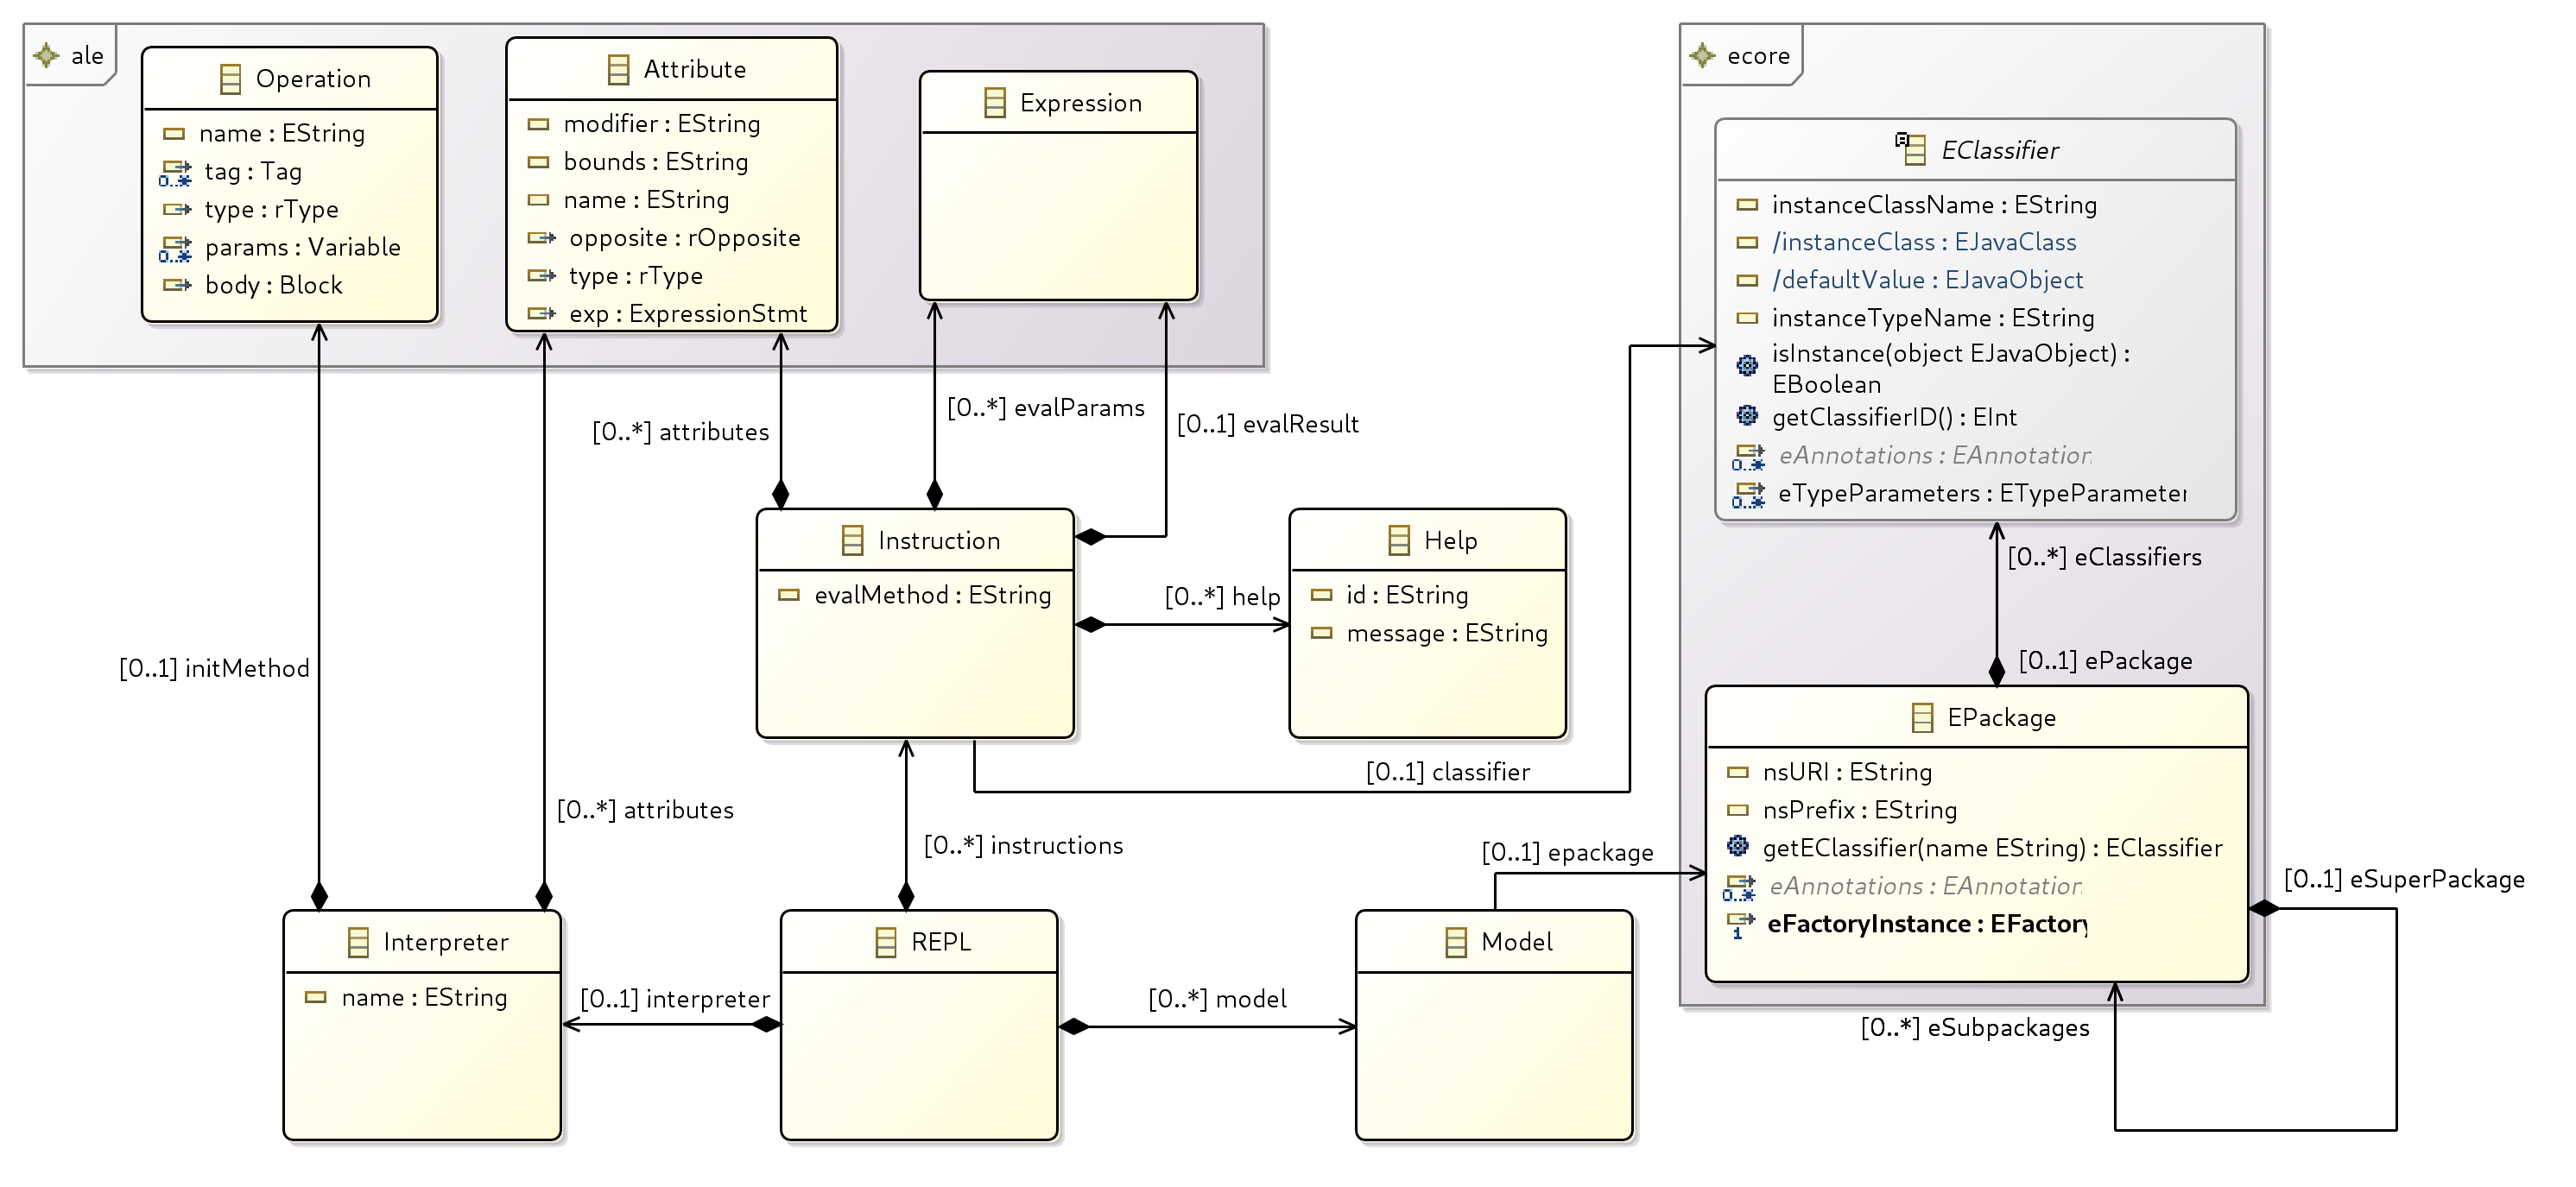
\includegraphics[width=.95\linewidth]{figures/visitor2repl_class_diagram.png}
	\caption{ReplDefinition metamodel}
	\label{fig:ReplDefinitionMetamodel}
\end{figure*}

We provide two concrete syntax to populate the model conform to the \textit{ReplDefinition} metamodel: a dedicated DSL, and additional annotations to ALE. This model represents the required information to drive the transformation of the DSL specification. 

\paragraph{Using a new DSL:}

The first concrete syntax is a new DSL built as an extension of ALE. Fig.~\ref{fig:repltransfo} shows the definition of the REPL for the \emph{Logo} language. 

The first part defines the entry points, associated outputs and help messages.  It defines two new entry points: Statement::execute and Expression::compute. It also defines their associated outputs to display: \textit{logo\_repl.turtle.toString()} and \textit{output.toString()} (\textit{output} refers to the actual value possibly returned by the entry-point). Finally we could define the help associated with these entry points (it has been done only partially in the Logo example). % \todo{ca serait bien de donner un example ici}

The second part specifies the \textit{Interpreter}, the specialization of its context of execution and its initialization.   
\textit{Interpreter} will serve as the starting point of the execution of the REPL and will manage the future instructions.
It will contain the same kind of runtime data as the entry-point of the base DSL, which will define the global context of the REPL. In the case of \textit{Logo}, this means the turtle graphics, and a symbol table used to define procedures (using a symbol table for this is simply a design choice of the language engineer). In order to initialize this global context, the initialization method of the interpreter will also be the same as the base DSL.

%In the current case, it defines a new execution context with two attributes \textit{Turtle} and \textit{SymbolTable} and defines their setup. These types exist in the current operational semantics. 

\begin{figure}[t]
	\centering
	\lstset{%
	    basicstyle=\scriptsize,
	    frame=single,
	    morekeywords={extend, as, interpreter, attribute, initmethod, instruction, output, help},
	    emph={syntaxmetamodel},
	    emphstyle=\itshape
	}
\begin{lstlisting}
extend http://www.gemoc.org/logo as logo

instruction logo.Statement:
    help right "Turn turtle of 'p' degrees to the right" 
    help forward "Move turtle of 'p' units forward" 
    execute(logo_interpreter.turtle, logo_interpreter.st)
        => logo_interpreter.turtle.toString();
instruction logo.Expression:
    compute(logo_interpreter.st)
        => output.toString();

interpreter logo_interpreter {
    attribute Turtle turtle;
    attribute SymbolTable st;
    initmethod def void init() {
        self.turtle := Turtle.create();
        self.turtle.xpos := 0.0;
        /* ... */
        self.st := SymbolTable.create();
        self.st.init();
    }
}

	\end{lstlisting}
	\caption{Example of ReplDefinition model for Logo}
	\label{fig:repltransfo}
\end{figure}

%As such, we chose to include them in the semantics, directly on the right operation.
\paragraph{Using annotations}

The same kind of information can be defined directly within the existing ALE operational semantics using a set of annotations.  We provided the language engineer with the following annotation:
\begin{alltt}
    @repl\textcolor{gray}{__outputtarget}\textcolor{lightgray}{__outputcall__...}
\end{alltt}
The output specification here is optional, and represents either an attribute read or a method call on a semantic object from the global context, or on the result of the operation being annotated. Note that the syntax is based on underscores because of limitations of the ALE language, which only supports identifiers as annotations.
Using two underscores as the separator allows for compatibility with semanics using either camel case or snake case for identifiers.

The language engineer can also set the help message to display by using a \textit{javadoc} like comment:
\begin{alltt}
    \textcolor{gray}{/**
     * keyword: Help message
     */}
\end{alltt}

In the base semantics for \textit{Logo}, the only additions besides the optional help messages were the two following annotations (cf. Github repository):
\begin{itemize}
    \item \verb|@repl_turtle_toString| for the \verb|execute| operation of \textit{Statement}
    \item \verb|@repl_output_toString| for the \verb|compute| operation of \textit{Expression}
\end{itemize}


\begin{figure}[t]
	\centering
	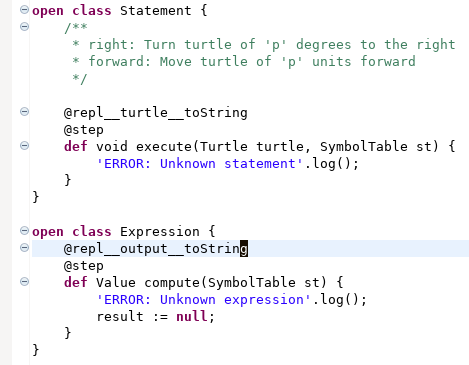
\includegraphics[width=\linewidth]{figures/annotations.png}
	\caption{ReplDefinition annotations used on Logo language}
	\label{fig:ReplDefinitionAnnotation}
\end{figure}

Fig~\ref{fig:ReplDefinitionAnnotation} shows a code excerpt from the operational semantics of the Logo language extended with the proposed annotations to define the information required to complement the DSL specification with an interactive programming environment. The set of annotations is however less expressive than the DSL. Indeed a language engineer might want to use a more complex expression as the output of an instruction or specialize the execution context for the REPL, which could not be done through annotations.
One could still choose to modify the behavior of the base semantics by adding a new ALE operation that could then contain any kind of ALE expression, and call it in the annotation.
This new operation could not, however, have access to the global context of the interpreter, nor to the intermediary results.

Based on this information, the DSL specification can be transformed so that a REPL can be derived and used by interactive computer programming environments. It is defined in three steps \textsc{i)} Abstract Syntax Tree transformation, \textsc{ii)} Concrete Syntax transformation, \textsc{iii)} Operational semantics transformation. The next subsections detail these three transformations applied on the original DSL specification. Finally, we present the generic REPL interface provided and the clients defined as interactive computer programming environments: a language shell and a notebook interface. 

%For this reason, we start by generating an intermediary transformation model written with a custom DSL (\textit{V2R}) that is openly editable (even though this is not necessary to obtain a working REPL).

%\subsection{V2R transformation model}



%\subsection{Grammar specification transformation}

%Using the annotated semantic and the definition of the abstract syntax, our tool generates a transformation model that defines all the mappings between the two languages.

%An example can be seen in figure~\ref{fig:v2r} with the language \textit{Logo}.


%Next are the instructions.
%For each \textit{repl} annotation from the semantic, the transformation model will include a mapping between the annotated method, actual parameters found from the runtime data of the interpreter, and optionally the expected outputs as defined in the annotation.

\subsection{Abstract syntax transformation}

\begin{figure}[t]
	\centering
	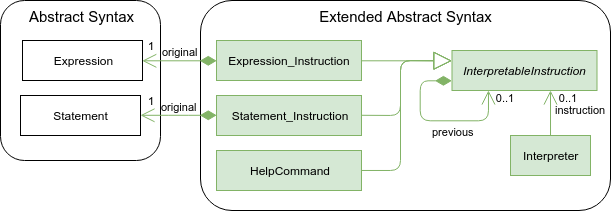
\includegraphics[width=\linewidth]{figures/sle_abstract_syntax.png}
	\caption{Abstract Syntax extension for Logo}
	\label{fig:as}
\end{figure}

During the DSL specification transformation process, we first complement the abstract syntax with additional concepts.

We first define \textit{Interpreter} as the REPL entry-point. It owns a reference to the abstract class \textit{InterpretableInstruction} which will be set during the execution to always target the current instruction.

\textit{InterpretableInstruction} also has a containment to itself, which creates a linked list of the previously executed instructions, hence keeping the whole execution history in a single resource.
For each instruction \textit{I} defined in the \emph{ReplDefinition} model, the new abstract syntax will include an adapter \textit{I\_Instruction} extending \textit{InterpretableInstruction}.
Another instruction is the \textit{HelpCommand}.

An example of the additions made for \textit{Logo} can be seen in Fig.~\ref{fig:as}.
The instructions that correspond to the new entry-points are \textit{Statement} and \textit{Expression}.

\subsection{Concrete syntax transformation}

The second step in our approach is to extend the existing concrete syntax to parse alternatives corresponding to the newly defined instructions.
As such, for each instruction \textit{I}, we retrieve the corresponding rule from the base grammar of the DSL and we reuse it for the newly defined adapter \textit{I\_Instruction}.
The parsing rule \textit{InterpretableInstruction} manages this part.

Another rule is created in order to instantiate an interpreter.
Then, the grammar entry-point will be the parsing rule \textit{EntryPoint} that will call either \textit{Interpreter}, \textit{InterpretableInstruction} or \textit{HelpCommand} if the user asks for help on a specific subject.

We also add a custom scope provider in order to resolve the cross references between the previously executed instructions and the current one.
When trying to resolve a cross reference, this scope provider will browse through the linked list of the previous instructions.
If nothing was found, it will finally turn to the resolution mechanisms of the base grammar.

One of the limitations of this specific implementation is that we use the default Xtext parser to parse single statements.
As such, we do not support non context-free grammars.
If the language has two semantically different instructions that use the same notation, only one of them can be made into an entry-point.
Some possible ways to support non context-free grammars would be:
\begin{itemize}
  \item to use a custom parser that could build a context from the previously executed instruction (which might add unwanted side effects)
  \item or to allow the language designer to modify the keywords used by some grammar rules, in order to remove potential conflicts
\end{itemize}

Fig.~\ref{fig:cs} depicts an organization of the different artifacts related to the concrete syntax extension of the language \textit{Logo}, while Fig.~\ref{fig:ecs} details the corresponding Xtext production rules.

\begin{figure}[t]
	\centering
	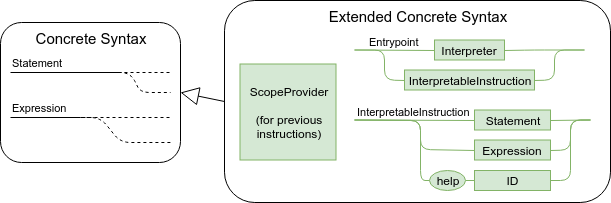
\includegraphics[width=\linewidth]{figures/sle_concrete_syntax.png}
	\caption{Concrete Syntax extension for Logo}
	\label{fig:cs}
\end{figure}

\begin{figure}[t]
	\centering
	\lstset{%
	    basicstyle=\scriptsize,
	    frame=single,
	    morekeywords={returns, repl, attribute, initrepl, instruction, output},
	    emph={syntaxmetamodel},
	    emphstyle=\itshape
	}
\begin{lstlisting}
// Import existing Logo definition. 

EntryPoint returns ecore::EObject:
  InterpretableInstruction | Interpreter;

InterpretableInstruction:
  {Statement_Instruction} original=Statement
    | {Expression_Instruction} original=Expression
    | {HelpCommand} 'help' command=ID;
  
Interpreter:
  {Interpreter}
	\end{lstlisting}
	\caption{Generated extended grammar definition for Logo}
	\label{fig:ecs}
\end{figure}



\subsection{Semantics transformation}

Last, we transform the DSL semantics to incorporate the new execution context and flow management, and to enable the new instructions to be executed.

Here, we handle operational semantics written in ALE.
ALE is a language that allows to re-open classes from Ecore metamodels to statically introduce fields and operations at design time.
By using the \textit{open class} syntax, we can define the behavior for the classes we added in the syntax, and drive the execution with \textit{@init} and \textit{@main} annotations on operations.

We define the runtime data of the execution context and the initialization of the \textit{Interpreter} entry-point as described in the \emph{ReplDefinition} model.
When executed, the interpreter will call the operation \verb|interpret| on the instruction it is currently referencing.

Every instruction adapter takes care of the mapping defined in the \textit{ReplDefinition} model: they become a wrapper that will call the original execution method of the statement or expression, possibly with the right parameters (the interpreter's execution context) and retrieve and display the expected outputs as described in the model.

Fig.~\ref{fig:sem} describes the overall execution flow for the language \textit{Logo}, while Fig.~\ref{fig:esementics} shows the generated ALE code corresponding to this execution flow. The Interpreter, its initialization method and specialized execution context are derived from the information provided by the language engineer in the \emph{ReplDefinition} model (see section \ref{sec:v2rmetamodel}). For each new entry point, an operation is added to manage the semantics. A new operation is also added to the new \textit{HelpCommand} meta-class. 

\begin{figure}[t]
	\centering
	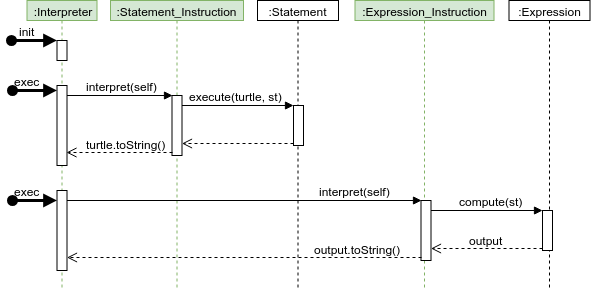
\includegraphics[width=\linewidth]{figures/sle_semantics.png}
	\caption{Overall execution flow for Logo}
	\label{fig:sem}
\end{figure}

\begin{figure}[t]
	\centering
	\lstset{%
	    basicstyle=\scriptsize,
	    frame=single,
	    morekeywords={returns, class, @init, @main,  open, void, def},
	    emph={syntaxmetamodel},
	    emphstyle=\itshape
	}
\begin{lstlisting}
open class Interpreter {
  logolang::Turtle turtle;
  logolang::SymbolTable st;

  @init
  def void init() {
    self.turtle := logolang::Turtle.create();
    self.turtle.xpos := 0.0;
    self.turtle.ypos := 0.0;
    self.turtle.direction := 0.0;
    self.turtle.pendown := false;
    self.turtle.canvas := logolang::Canvas.create();
    self.turtle.canvas.segments := Sequence{};
    self.st := logolang::SymbolTable.create();
    self.st.init();
  }

  @main
  def void run () {
    self.instruction.interpret(self);
  }
}

open class Expression_Instruction {
  def void interpret(Interpreter logo_repl) {
    ecore::EObject output := 
      self.original.compute(logo_repl.st);
    output.toString()?.log();
  }  
}

open class Statement_Instruction {
  def void interpret(Interpreter logo_repl) {
    self.original.execute(logo_repl.turtle, logo_repl.st);
    logo_repl.turtle.toString()?.log();
  }
}

open class HelpCommand {
  def void interpret(Interpreter logo_repl) {
    // Call help method of the node
  }
}

	\end{lstlisting}
	\caption{Generated extended operational semantics for Logo}
	\label{fig:esementics}
\end{figure}


\subsection{REPL Interface and Interactive Environments Examples}

%%%% BEGIN: FROM SECTION 3 %%%%

\begin{figure}[t]
	\centering
	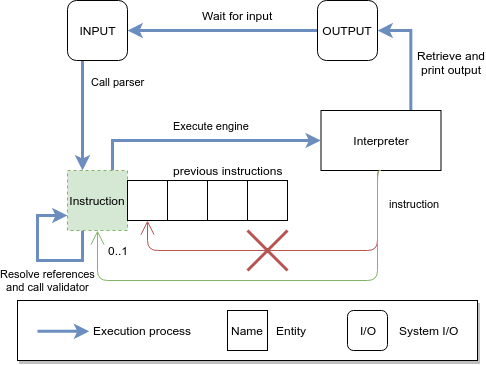
\includegraphics[width=0.9\linewidth]{figures/sle_engine_wrapper.png}
	\caption{REPL execution}
	\label{fig:engine-wrapper}
\end{figure}

Having applied the aforementioned transformation process, the DSL is complemented with a multi entry points parsing of interpretable instructions. In order to build an interactive environments on top of it, we provide a generic REPL interface protocol and its underlying systematic execution framework (cf. Fig.~\ref{fig:engine-wrapper}):
%The generated REPL semantics is the following:
\begin{samepage}
\begin{enumerate}
    \item Create an interpreter and initialize it
    \item \label{loop} Read the user input
    \item Parse it as an instruction
    \item Retrieve the previous instruction and store it
    \item Swap the instruction of the interpreter for the new one
    \item Run the interpreter
    \item Print the relevant output
    \item Go back to step \ref{loop}
\end{enumerate}
\end{samepage}

%%%% END: FROM SECTION 3 %%%%

\begin{figure}[t]
	\centering
	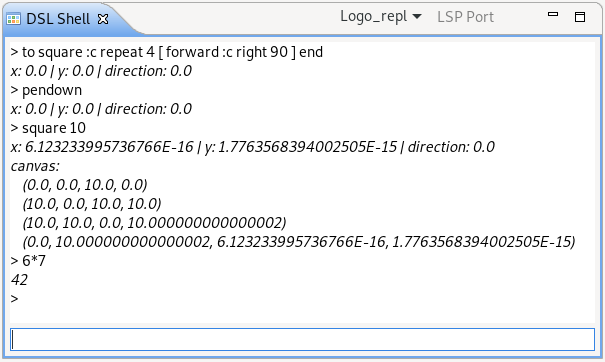
\includegraphics[width=\linewidth]{figures/logo_shell.png}
	\caption{Eclipse shell running with Logo REPL}
	\label{fig:logo_shell}
\end{figure}

From the new generated DSL specification, we automatically generate the entire GLUE code for integration with two technical environments: Eclipse and Jupyter. 
For the first one, we provide a plugin including an eclipse view hosting a shell to communicate with the Interpreter.  This generic view declares an Eclipse extension point type including among others the name of the REPL language and the qualified name of the interpreter class. 
Each REPL language declares this extension point. The generic view allows REPL users to select the desired DSL and then start an interactive session. This session keeps track of the executed instructions and offers the ability to reset the interpreter or cancel the last instructions thanks to the environment provided by Gemoc. The Language Server Protocol (LSP\footnote{\url{https://langserver.org/}}) support provided by Xtext enables intelligent completion within the Shell. Figure~\ref{fig:logo_shell} shows a screenshot of this integration within Eclipse for the Logo language. 

For Jupyter, an editor specific to ipynb files (Jupyter notebook) has been created and manually integrated into Jupyter. The purpose of this editor is to replace the default code cell editor (ace editor\footnote{Cf. \url{https://ace.c9.io/}}) with the monaco text editor\footnote{Cf. \url{https://microsoft.github.io/monaco-editor/}}. The latter has the advantage of natively supporting LSP in order to allow completion, error reporting, etc. A generic glue code has been added to adapt between Jupyter's Kernel concept and GEMOC's execution engine to control the execution of interpreters. Thus for each new REPL, a connection file defining the connection URL to the GEMOC execution engines of this REPL is generated. A descriptor is also generated for Jupyter to register this new kernel. 


\begin{comment}
\begin{figure}[t]
	\centering
\begin{lstlisting}[language=json]
{
 "argv": ["python3", "-m", "REPL.kernel",
          "-f", "{connection_file}"],
 "display_name": "LOGO REPL",
 "language": "logo"
}
\end{lstlisting}
\end{figure}
\end{comment}

On the GEMOC side, a class allowing to interface with a ZeroMQ message oriented middleware is created and makes the link with the execution interface of the GEMOC engine and the current REPL. The main advantages of the GEMOC integration is to leverage its execution trace management, debugging facilities and concurrency model management (e.g., to start from any cell or finely control the flow of execution of the cells.).


%(C'est un peu applatti)
%Les attributs et la méthode init c'est exactement ce que j'ai défini dans le V2R (vu que c'est du ALE de base)
%Et pour le générer dans le V2R, je me suis basé sur l'annotation init de base



%\subsection{REPL Semantics}

%Since we use a regular single-program execution engine, we need to add a mechanism in order to retrieve and reuse the runtime context, in order to get a proper interactive environment.
%It is also necessary to have the read-eval-print-loop behaviour that it lacked.
%As such, we decided to implement this in a wrapper for the base execution engine.

%The first action of this wrapper is to create and initialize the actual engine.
%We consider that the global context for future instructions should be defined during this phase, by calling an initialization method from the semantic.

%Then comes the REPL part: the wrapper manages buffers for both inputs and outputs, and will continuously wait for new input before processing it as intended.
%Having received a new instruction as a string, it parses it to an actual executable instruction by following the rules of the previously generated syntax (Section~\ref{transformation}).
%The input can also be an internally defined command: in our case, we have \textsc{exit} and \textsc{help}.
%If there were previously executed instructions in the current instance, the instruction gets enriched with the whole history.
%Post-parsing operations like cross references resolution and validations are manually applied, then the instruction gets passed to the actual engine with the runtime context (in the case of the ALE engine, the context is kept by the engine as long as we don't manually reset it).
%At last, the wrapper captures the outputs and errors from the whole process and stores them in its buffers.


%\section{Interactive Computer Programming Environment}

\subsection{Application to the GEMOC Studio}

%\todo[inline]{Presentation of the GEMOC Studio}

In order to test our approach, we made an implementation integrated within the environment provided by the GEMOC Studio.
Our goal was to obtain a generic process that could be applied to any DSL defined with the EMF/XText technical stack that also uses ALE to define its operational semantics.

%\todo[inline]{Language shell}

\section{Evaluation}
\label{sec:evaluation}

To address the four challenges identified in Section \ref{approach}, we propose an approach to automatically generate an interactive computer programming environment from a DSL specification and an identification of the execution entry points for this REPL. A first level of validation consists in applying our approach on other DSLs, namely \textit{MiniJava} and \textit{ThingML}, and to reflect on the lessons learnt. 
   

%In addition to Logo, we applied our approach on two other DSLs.

\textit{MiniJava} is a subset of the general purpose language \textit{Java} that was created for teaching purposes, since \textit{Java} was considered too intimidating for students on various aspects \cite{Roberts:2001:OM:364447.364525}. The first implementation of \textit{MiniJava}, released in 2001, was also shipped with a REPL.  This DSL offer a good support to learn Java and test APIs as introduced in Section~\ref{motiv}.

We started from an existing implementation in EMF/Xtext/ALE\footnote{Cf. \url{https://github.com/manuelleduc/ale-lang/tree/master/languages/minijava}}.
This specific implementation is a large one, with 80 meta-classes and 200 attributes in the abstract syntax, 170 lines of Xtext for the grammar, and more than 1140 lines of ALE as operational semantics.
In order to use real life APIs, we decided to add a support for native \textit{Java} calls through the Java JSR-223 API\footnote{Cf. \url{https://docs.oracle.com/javase/8/docs/technotes/guides/scripting/prog\_guide/api.html}}. 	JSR-223 is a standard API for calling scripting frameworks in Java. It is available since Java~6 and aims at providing a common framework for calling multiple languages from Java. 

We selected nine execution entry-points: Type declarations, Method definitions, Statement blocks, Variable declarations, Assignments, For loops, While loops, Conditions, and Expressions. This means that we added nine \verb|@repl| annotations, including one with a specific output for the expressions. Considering the initial size of the DSL specification, these additions are only nine more lines in the semantics, which can be estimated as a modification of $0.6\%$ to generate a REPL for the existing DSL.

%In the implementation that we used, the scoping was managed by a Xtext \textit{ScopeProvider} and the access rights were enforced by a Xtext \textit{Validator}. However, these two elements didn't follow a pure interpreter pattern implementation. The \textit{ScopeProvider} assumed that a statement would only exist within a \textit{Method}, a \textit{Block} or a \textit{For} loop condition, and the \textit{Validator} expected that every element would have a class in its hierarchy. As these were not respecting our initial hypothesis, we had to make them more defensive by adding \verb|null| checks before we could use them. When written defensively, scopes and visibilities work as intended for the generated REPL.

We also added both a Xtext \textit{ScopeProvider}, to manage the scoping, and a Xtext \textit{Validator}, to enforce access rights, to the base definition of \textit{MiniJava}.
Having these two new elements written with the pure interpreter pattern inside the DSL definition was not an issue, and they both work as intended for the generated REPL.

The second DSL is an ALE implementation of \textit{ThingML}. ThingML\footnote{Cf. \url{https://github.com/TelluIoT/ThingML}} is a domain specific modeling language, that combines well-proven software modeling constructs for the design and implementation of distributed reactive systems:

\begin{itemize}
    \item statecharts and components (aligned with UML) communicating through asynchronous message passing,
\item an imperative platform-independent action language,
\item specific constructs targeting IoT applications.
\end{itemize}

The ThingML language is supported by a set of tools, which include editors, transformations (\emph{e.g.,} export to UML) and an advanced multi-platform code generation framework, which supports multiple target programming languages (C, Java, Javascript). Recently a simulator has been designed to emulate the distributed system behavior. The abstract syntax contains 88 meta-classes, for a total of 240 model elements. The grammar definition is more than 450 lines long, and writing the operational semantics in ALE require more than 1800 lines.

Being a dataflow language, it was an interesting case study for us since our approach was mainly aimed at imperative DSLs.

In a \textit{ThingML} program, a language user can define types and protocols, with some of those types being ``things'' that can declare functions and state machines, before instantiating them inside configurations. A configuration of connected things is a dataflow, and the operational semantics of \textit{ThingML} execute it for as long as they have steps to execute.

The syntax of the DSL offers a way to describe complete dataflows, and our approach enables the definition of partial programs.
However, the concept of partial dataflows is debatable. %\todo{à enrichir pourquoi est ce débattable au minimum mais une ref vers le débat}
Since ThingML uses named elements in a configuration, we could use them as valid execution entry-points, but a smaller granularity would not make sense:
\begin{itemize}
    \item We could have instantiations and connections between things outside of configurations, but this would mean either that we execute a partial flow from the beginning after each change, or that \textit{ThingML} defines an \verb|execute| instruction (and it does not). Running several configurations is honestly just as good.
    \item The statements used in functions could be available, but at best they could only be used to interact with completely executed configurations (and their instances if the concrete syntax provided a definition for qualified names), which would be of limited use.
    \item With the two above, we could actually end up with a complete imperative  language, but it would be too far away from the original \textit{ThingML} to stay in the scope of what we want to provide.
\end{itemize}

As such, we decided to use the following 3 entry-points: Type definition, Protocol definition, and Configuration declaration (and execution). They correspond to 3 more lines in the semantics, which represent $0.12\%$ of the total DSL specification.
Our \textit{ThingML} REPL makes it possible to split a program between elements definition and several configuration executions.
However, there are a lot more interesting aspects to an interactive environment for a dataflow language: altering an already existing dataflow with new nodes and transitions, or controlling the execution step by step for example.

\subsection*{Lessons learned}

This experiment on two DSL specifications defined by other language engineers allowed us to verify several points, and to evaluate our initial RQ and associated four challenges. 

The first lesson learned is the ability of our approach to be used on different DSLs as long as these specifications conformed to a certain number of expectations. The language engineer can specify the new entry points of the DSL, the associated outputs and the associated help messages in an expressive way. The effort to define these entry points remains low compared to the level of reuse of the abstract syntax, the grammar and the operational semantics. 
Such an approach of automated transformation allows a language engineer to have significant confidence in the semantics preservation of the original DSL. Focusing all the tools associated with a DSL only on its specification is an important way to facilitate the evolution of all these artifacts, and in particular the associated REPL. 
The assumptions made about the form of the implementation of static semantics, the operational semantics, and the different scoping rules are a bit strong. This means that two things are required at the moment: The definition of new entry points must be done by a language engineer and it is required to be able to access the DSL specification in case of issues to correct the parts that do not fully respect the assumption of a pure interpreter design pattern. Finally, if the approach perfectly fits the generation of interactive computer programming environments for imperative languages, many perspectives are opening up in the case of declarative or dataflow languages, and they lead to considering new opportunities for the interactive parts of these kinds of languages. 


%1. Possible de générer un REPL de manière automatique. 

%. Volume d'information à définir pour permettre la génération automatique assez faible et faible en ratio du volume d'élément réutilisé dans le 

%3. Assomption un peu forte qui force ce travail de définition d'un REPL à être exécuté par un language designer expert. 

%4. Nombreuses perspectives ouvertes sur la notion de dataflow. 



\section{Related works}
\label{sec:rw}

Various generic frameworks have been proposed in the last decade to integrate language REPLs, either for education purpose (\emph{e.g.,} Repl.it\footnote{cf. \url{https://repl.it}}) or scientific computing (\emph{e.g.,} Jupyther\footnote{cf. \url{https://jupyter.org}}). In all cases, a specific implementation of the language must be provided. While the implementation is time consuming, this is also error prone and needs to be aligned with the initial semantics of the language. 

Bacat\'{a} has been recently proposed to automatically derive a new kernel for Jupyter from a DSL specification defined within the language workbench Rascal \cite{Merino:2018:BLP:3276604.3276981}. While all the implementation is automatically generated from the specification, the specification (i.e., the syntax and the semantics) has to be defined specifically for supporting a REPL. 

Our approach automates the transformation from an initial specification for a textual interpreted DSL to a new specification and the underlying language implementation for being integrated into an interactive computer programming environnement. The resulting implementation can be integrated into either a simple language shell or more complex environments such as Notebooks. To the best of our knowledge, there is no related work addressing the specific challenge of automatically transforming a language syntax and semantics to support interactive programming (\emph{i.e.}, multiple execution entry-points, and management of the execution context and flow).

\section{Conclusion and future work}
\label{sec:conclusion}

We describe in this paper an approach to automatically transform an existing specification of a textual and interpreted DSL, into a new specification that drives the development of an interactive computer programming environment. From additional information about the allowed entry points and the expected outputs when executed, we describe how to transform the grammar specification and the operational semantics specification so that we can have multiple execution entry points, and a sound and extensible management of the execution context and flow. We also define a unified interface to be used from different interactive environments such as a language shell and a notebook interface. The implementation and the evaluation have been done in the GEMOC Studio, but the proposed approach could be implemented in other language workbenches. 

This approach opens up various perspectives. While our approach is currently expecting operational semantics in the form of an interpreter, we would like to extend it in the future to also cover translational semantics in the form of a compiler. We would also investigate the support of a seamless interoperability \cite{coulon:hal-01889155} between the interactive computer programming environments and the initial environment. In the long term, we would like to investigate polyglot interactive environments offering a seamless integration of heterogeneous languages.




%This paper provides a first result around the work of providing the ability to automatically create an interactive computer programming environment from a language specification. It shows that from metadata defined by the language designer on i) the program entry points to be considered, ii) the outputs for these entry points, it is possible to construct a first level of REPL with the condition that the specification of the REPL respects some assumptions. 

% How to tackle denotational semantic definitions? How to support relaxed grammar rules in which incomplete fragments of instructions are tolerated. How to allow the composition of the interactive computer programming environment by sharing the context between several interpreters? These open challenges would represent the next breakthroughs of our work on REPL generation.

%%
%% The next two lines define the bibliography style to be used, and
%% the bibliography file.
\bibliographystyle{ACM-Reference-Format}
\bibliography{bibliography}

\end{document}
